\section{Descripción general del sistema}

El diseño implementado corresponde a un sistema UART extendido con capacidades de procesamiento mediante una \textbf{Unidad Aritmético-Lógica (ALU)}. El bloque superior \texttt{top} integra todos los módulos que lo componen y define el flujo de datos completo desde la entrada serie (\texttt{rx}) hasta la salida (\texttt{tx}).

\subsection{Bloque \texttt{top}}
El módulo \texttt{top} actúa como entidad principal, interconectando:
\begin{itemize}
    \item El generador de baudios, encargado de derivar la señal de muestreo \texttt{sample\_tick}.
    \item El receptor UART (\texttt{uart\_rx}), que reconstruye bytes a partir de la señal serie entrante.
    \item Dos memorias FIFO: una para los datos recibidos y otra para los datos a transmitir.
    \item El transmisor UART (\texttt{uart\_tx}), que serializa los datos de salida.
    \item El módulo \texttt{interface}, encargado de interpretar los bytes recibidos como operación y operandos, y enviar los resultados a la FIFO de transmisión.
    \item La ALU, que realiza las operaciones aritméticas y lógicas definidas.
\end{itemize}

\subsection{Esquemático general}
La Figura~\ref{fig:uart-general} muestra un diagrama de bloques típico de un sistema UART completo, donde se observa la integración del generador de baudios, los bloques de transmisión y recepción, y las memorias FIFO.

\begin{figure}[H]
    \centering
    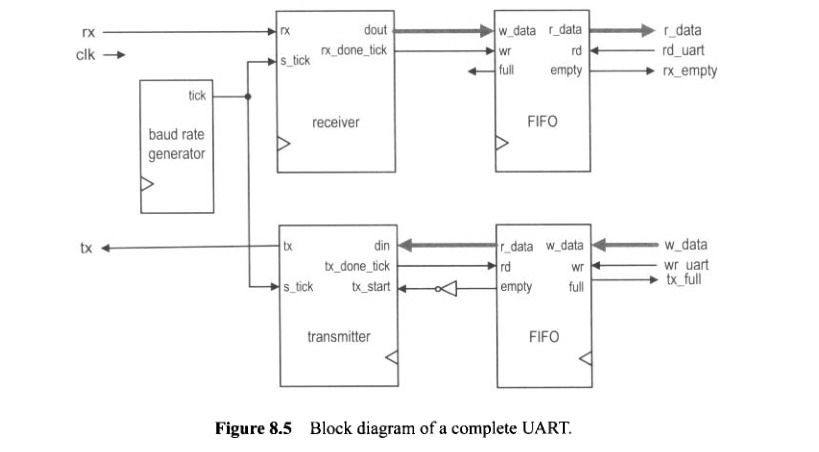
\includegraphics[width=0.75\textwidth]{img/completeUART.jpeg}
    \caption{Diagrama de bloques de un UART completo \cite{libroUART}.}
    \label{fig:uart-general}
\end{figure}

\subsection{Flujo de datos}
El flujo de información en el sistema sigue la siguiente secuencia:
\begin{enumerate}
    \item Los datos ingresan por la línea \texttt{rx} y son muestreados por el \texttt{uart\_rx}.
    \item Los bytes reconstruidos se almacenan en la \textbf{FIFO RX}.
    \item El módulo \texttt{interface} extrae los datos de la FIFO y organiza los tres bytes requeridos: código de operación, operando A y operando B.
    \item La ALU procesa estos valores y genera un resultado.
    \item El resultado se escribe en la \textbf{FIFO TX}.
    \item Finalmente, el \texttt{uart\_tx} serializa el dato y lo envía por la línea \texttt{tx}.
\end{enumerate}
